\documentclass[a4paper, 12pt]{article}

%\usepackage{cmap}
\usepackage[T2A]{fontenc}
\usepackage[utf8]{inputenc}
\usepackage[english, russian]{babel}
\usepackage{graphicx}
\usepackage[top=1in, bottom=1in, left=3.2cm, right=2.6cm]{geometry}
\graphicspath{./}
\usepackage{biblatex}
\addbibresource{lib.bib}
\linespread{1.5}
\usepackage{ragged2e}
\justifying
\usepackage{listings}
\usepackage{color}
\usepackage{amsmath}


\begin{document}
	
\begin{titlepage}
	\fontsize{12pt}{12pt}\selectfont
	\begin{figure}[t!]
		\centering
		
\includegraphics[scale=0.8]{bmstu}
	\end{figure}
	
	\noindent\rule{15cm}{3pt}
	\newline\newline
	\noindent 
	ФАКУЛЬТЕТ 
	\underline{«Информатика и системы управления»} \newline
	
	\noindent КАФЕДРА \underline{«Программное обеспечение ЭВМ и информационные технологии»}\newline\newline\newline\newline\newline
	
	\centering {\Large \textbf{Отчет по лабораторной работе № 5}}
	\vspace{4mm}
	
	\centering {\Large \textbf{По курсу:} Моделирование
		\vspace{8mm}}
	\\ \centering {\Large \textbf{На тему:} Моделирование работы информационного центра}
	\vspace{20mm}
	
	
	\begin{flushright}
		{\small	\textbf{Студент:}\\ Турсунов Жасурбек Рустамович \\ \textbf{Группа:} ИУ7-76Б
			\vspace{3mm}
			\\\textbf{Преподователь:} \\ Рудаков Игорь Владимирович }
	\end{flushright}
	
	\begin{center}
		\vfill
		Москва, \the\year
		~г.
	\end{center}
\end{titlepage}

\tableofcontents
\clearpage
\newpage


\section{{Задание}}

\hspace*{5mm} В информационный центр приходят клиенты через интервал времени 10 $\pm$ 2 минуты. Если все три имеющихся оператора заняты, клиенту отказывают в обслуживании. Операторы имеют разную производительность и могут обеспечивать обслуживание среднего запроса пользователя за 20 $\pm$ 5; 40 $\pm$ 10; 40 $\pm$ 20. Клиенты стремятся занять свободного оператора с максимальной производительностью. Полученные запросы сдаются в накопитель. Откуда выбираются на обработку. На первый компьютер запросы от 1 и 2-ого операторов, на второй – запросы от 3-его. Время обработки запросов первым и 2-м компьютером равны соответственно 15 и 30 мин. Промоделировать процесс обработки 300 запросов.
\hspace*{5mm} Для выполнения поставленного задания необходимо создать концептуальную модель в терминах СМО, определить эндогенные и экзогенные переменные и уравнения модели. За единицу системного времени выбрать 0,01 минуты.
\begin{figure}[h!]
	\centering 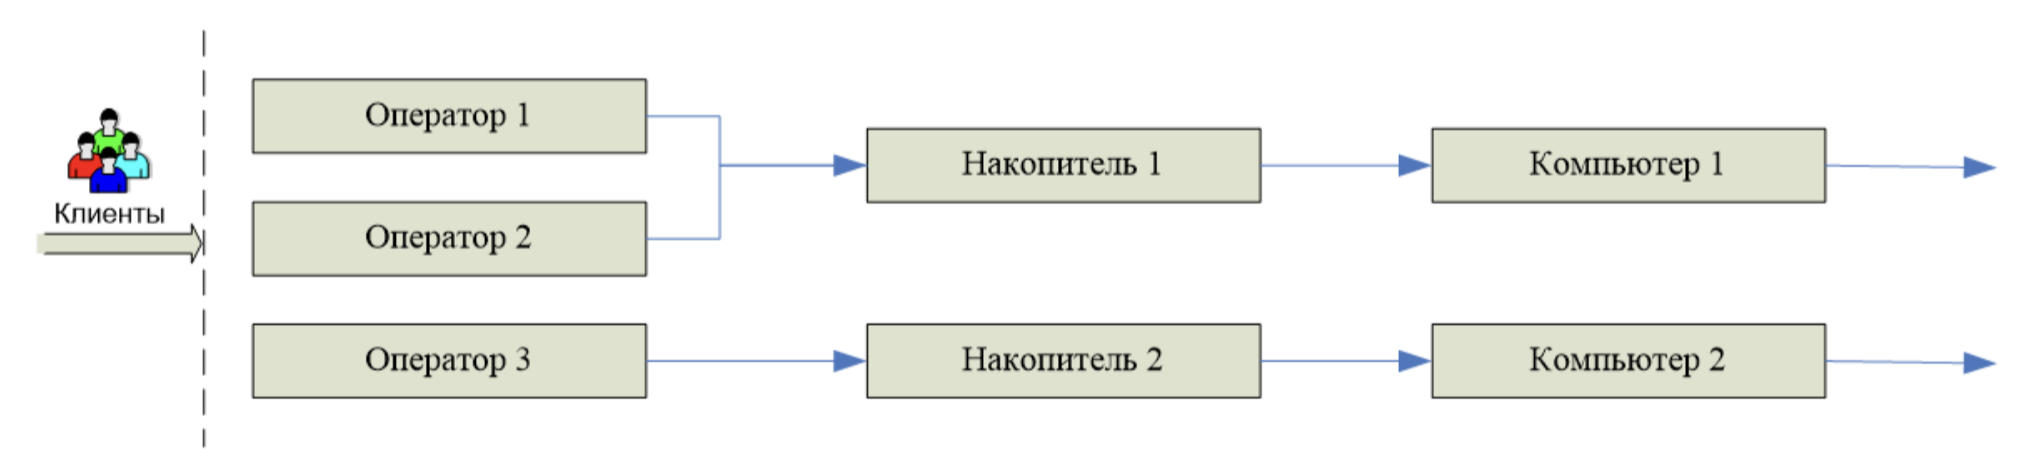
\includegraphics[scale=0.4]{schema}
\end{figure}

\section{{Теоритическая часть}}
\hspace*{5mm} В процессе взаимодействия клиентов с информационным центром возможно:
\begin{itemize}
	\item режим нормального обслуживания, т.е. клиент выбирает одного из свободных операторов, отдавая предпочтение тому у которого меньше номер;
	\item режим отказа в обслуживании клиента, когда все операторы заняты. 
\end{itemize}
\textbf{Переменные и уравнения имитационной модели }
\\ \hspace*{5mm} Эндогенные переменные: время обработки задания i-ым оператором, время решения этого задания j-ым компьютером.
\clearpage
\newpage
\hspace*{5mm}  Экзогенные переменные: число обслуженных клиентов и число клиентов, получивших отказ.
\begin{figure}[h!]
	\centering 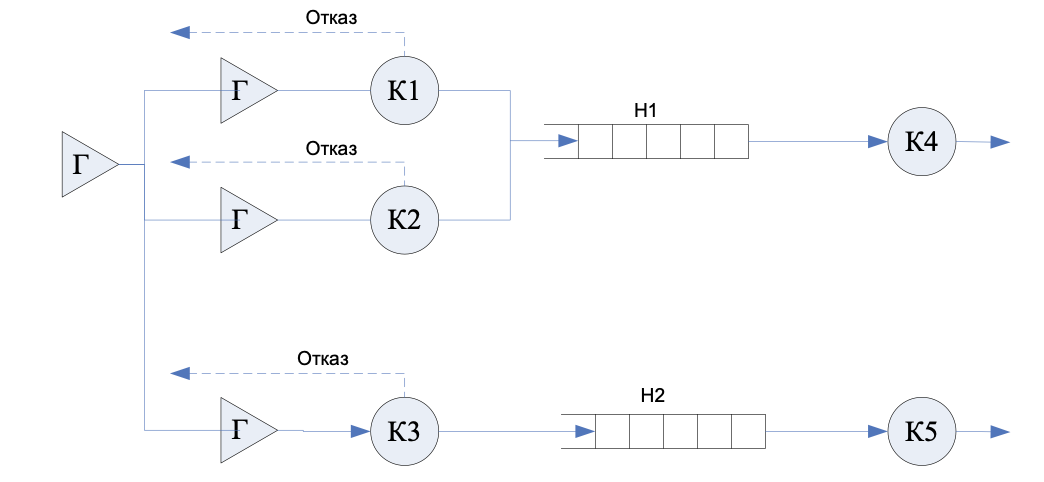
\includegraphics[scale=0.7]{schema1}
\end{figure}

\section{{Результаты}}
\begin{figure}[h!]
	\centering 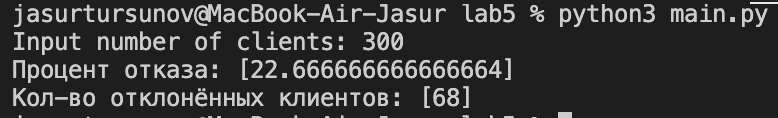
\includegraphics[scale=1]{300}
\end{figure}
\begin{figure}[h!]
	\centering 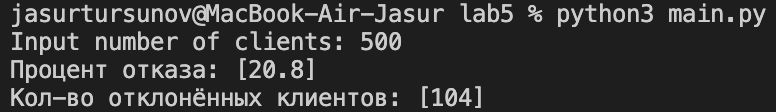
\includegraphics[scale=1]{500}
\end{figure}
\begin{figure}[h!]
	\centering 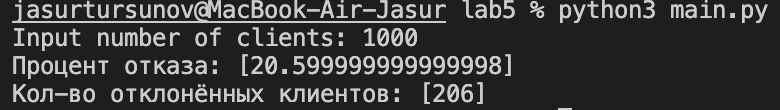
\includegraphics[scale=1]{1000}
\end{figure}

\section{Листинг кода}
\definecolor{codegreen}{rgb}{0,0.6,0}
\definecolor{codegray}{rgb}{0.5,0.5,0.5}
\definecolor{codepurple}{rgb}{0.58,0,0.82}
\definecolor{backcolour}{rgb}{0.95,0.95,0.92}

\lstdefinestyle{mystyle}{
	backgroundcolor=\color{backcolour},   
	commentstyle=\color{codegreen},
	keywordstyle=\color{magenta},
	numberstyle=\tiny\color{codegray},
	stringstyle=\color{codepurple},
	basicstyle=\ttfamily\footnotesize,
	breakatwhitespace=false,         
	breaklines=false,                 
	captionpos=b,                    
	keepspaces=true,                 
	numbers=left,                    
	numbersep=5pt,                  
	showspaces=false,                
	showstringspaces=false,
	showtabs=false,                  
	tabsize=4
}

\lstset{style=mystyle}

\begin{lstlisting}[language=Python, caption = Программная реализация работы информационного центра]
def event_mode(self):

	refusals = 0

	generated_requests = self.generator.num_requests

	generator = self.generator


	generator.receivers = self.operators.copy()

	self.operators[0].receivers = [self.computers[0]]

	self.operators[1].receivers = [self.computers[0]]

	self.operators[2].receivers = [self.computers[1]]


	generator.next = generator.delay()

	self.operators[0].next = self.operators[0].delay()


	blocks = [

		generator,

		self.operators[0],

		self.operators[1],

		self.operators[2],

		self.computers[0],

		self.computers[1],

	]


	while generator.num_requests >= 0:

		current_time = generator.next

		for block in blocks:

			if 0 < block.next < current_time:

				current_time = block.next


		for block in blocks:

			if current_time == block.next:

				if not isinstance(block, ProcessRequest):

					next_generator = generator.generate_request()

					if next_generator is not None:

						next_generator.next = \

						current_time + next_generator.delay()

					else:

						refusals += 1

					generator.next = current_time + generator.delay()

				else:

					block.process_request()

					if block.queue == 0:

						block.next = 0

					else:

						block.next = current_time + block.delay()


	return {"refusal_percentage": refusals / generated_requests * 100,

		"refusals": refusals}
\end{lstlisting}
\end{document}